\documentclass[varwidth=true, border=2pt]{standalone}

\usepackage{pgfplots}
\usepackage{tikz}
\usepackage{amsmath}
\usepackage{amssymb}

\usetikzlibrary{patterns}

\usetikzlibrary{calc,patterns,angles,quotes}

\newcommand{\R}{\mathbb{R}}

\begin{document}
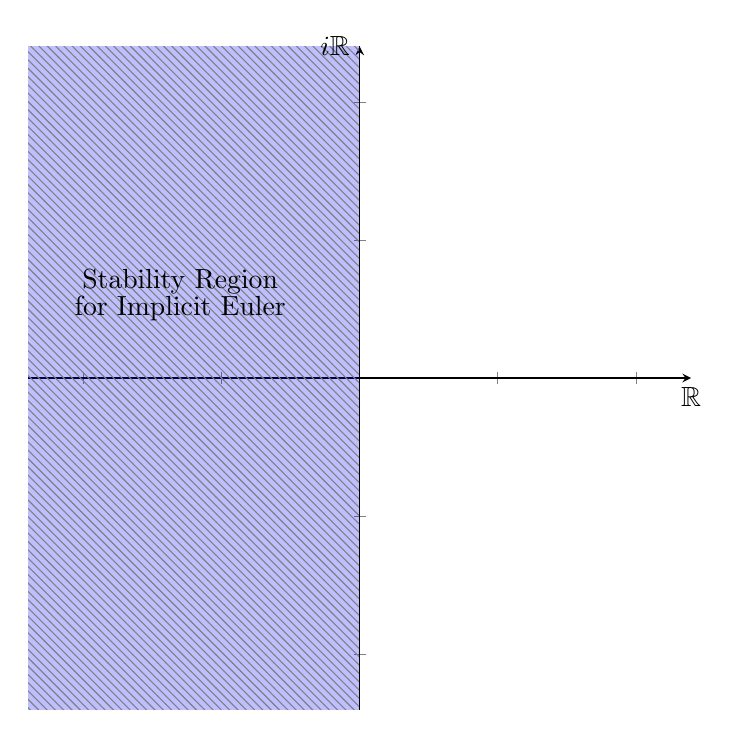
\begin{tikzpicture}
    \begin{axis}[
        legend pos=south east,
        axis x line=middle,
        axis y line=middle,
	every axis x label/.style={at={(current axis.right of origin)},anchor=north},
	every axis y label/.style={at={(current axis.above origin)},anchor=east},
	xticklabels=\empty,
	yticklabels=\empty
        grid = none ,
        width=10cm,
        height=10cm,
        grid style={dashed, gray!1},
        xmin=-1,
        xmax=1,
        ymin=-1,
        ymax=1,
        xlabel=$\R$,
        ylabel=$i \R$,
        enlargelimits=true,
        tension=0.08]

	\draw [fill=blue, opacity = 0.25] (axis cs: -2,2) rectangle (axis cs: 0, -2);
	\draw [pattern=north west lines, pattern color=gray] (axis cs: -2,2) rectangle (axis cs: 0, -2);
	\node (S1)  at (axis cs: -0.65,0.35) {Stability Region};
	\node (S2) at (axis cs: -0.65,0.25) {for Implicit Euler};

    \end{axis}
\end{tikzpicture}
\end{document}